\chapter{Marco teórico}

En este capítulo se presentan, de forma teórica, los conceptos y técnicas
necesarias para el desarrollo de este proyecto. Se comienza por delimitar
la problemática en el marco del NLP, posteriormente se presentan los
modelos de lenguaje y su aplicación a la problemática, así como la
descripción de la técnica de recuperación-generación aumentada que se empleará.
Por último se presentan conceptos adicionales necesarios para el desarrollo del proyecto,
así como trabajos relacionados en el área.

\section{Delimitación de la problemática}

El objetivo de este proyecto es desarrollar un asistente virtual tipo chatbot
que responda preguntas de documentos específicos. Si bien, un asistente
virtual inteligente se desempeña en diferentes áreas del NLP, este proyecto
se centra específicamente en el que se conoce como dar respuesta a preguntas
(QA, Question Answering).

En el contexto del NLP, se entiende por QA al desarrollo de sistemas que
permiten a los usuarios utilizar interfaces de lenguaje natural para formular
preguntas y recibir respuestas concisas \cite{pereira_systematic_2022}.
Estos sistemas pueden presentarse de diferentes formas, siendo las aplicaciones basadas
en modelos de lenguaje de gran tamaño (LLMs) las que predominan en el área.
El uso de LLMs hace posible la creación de sistemas que respondan
a preguntas de forma interactiva (IQA, Interactive Question Answering),
en los cuales el sistema puede entablar conversaciones con el usuario y responder
de forma dinámica \cite{biancofiore_interactive_2024}.

Una parte importante del QA es que, generalmente, funciona con ternas de
información: pregunta, contexto, respuesta. La pregunta y la respuesta
son secuencias de texto en lenguaje natural, y el contexto se refiere a
la información que empleará el modelo para contestar la pregunta, usualmente
el contexto también se encuentra en forma de texto, aunque puede tener
otras formas.

Dentro de los sistemas IQA y QA, existen diferentes elementos a evaluar,
sin embargo la evaluación de la respuesta es el parámetro fundamental en la
mayoría de ellos; para ello se emplean conjuntos de datos especializados que contienen
preguntas, su contexto y las respectivas respuestas, por ejemplo:
TREC (\textbf{T}ext \textbf{RE}trieval \textbf{C}onference)
\cite{noauthor_proceedings_2001}, Yahoo! (YH) \cite{zhou_learning_2016},
WikiQA \cite{yang_wikiqa_2015}, Standford Question Answering Dataset (SQuAD)
\cite{rajpurkar_squad_2016}, entre otras.


\section{Modelos de lenguaje de gran tamaño (LLMs)}

Para entender lo que es un LLM, primero es necesario presentar el concepto
de red neuronal artificial (ANN, Artificial Neural Network).
Una red neuronal artificial es un modelo dividido en capas de
procesamiento, donde cada capa se compone de nodos o neuronas. Cada neurona
recibe entradas ponderadas, les aplica una transformación y devuelve una
salida. En el modelo tradicional de red neuronal, conocido como
\textit{feedforward}, las salidas de cada capa sirven como entrada de la
siguiente, de esta forma la información se propaga
desde la capa de entrada, pasando por una o más capas ocultas hasta llegar
a la capa de salida, donde se obtiene el resultado final de la red.

Múltiples arquitecturas de ANNs han sido creadas con diferentes propósitos,
y a su vez, se han creado mecanismos que funcionan en conjunto con estas
redes para mejorar su desempeño en tareas específicas. En el contexto del
NLP uno de estos mecanismos es la \textit{atención}. Este mecanismo
fue introducido por Bahdanau et al. \cite{bahdanau_neural_2016} en el contexto
de la traducción de texto automática con el propósito de que la red neuronal
decida a qué partes de las oraciones prestar atención.
Si bien Bahdanau no empleó el término \textit{atención}, su propuesta fue
tomada por Vashwani et al. \cite{vaswani_attention_2017} para crear la
arquitectura del \textit{transformer} para crear una arquitectura basada
únicamente en mecanismos de \textit{atención} la cual se muestra en la figura
\ref{fig:transformer}.

\begin{figure}
    \centering
    \includegraphics[width = 0.55\textwidth]{\DirFigCdos/Transformer}
    \caption{Arquitectura \textit{transformer}.}
    \label{fig:transformer}
\end{figure}

El \textit{transformer} esta basado en una arquitectura del tipo
codificador-decodificador, es decir, una red neuronal divida en dos partes
cuyo objetivo es convertir una secuencia de texto a otra.
En su artículo, Vashwani et al. \cite{vaswani_attention_2017} definen
una función de \textit{atención} como un mapeo de una
\textit{query} y un conjunto de pares \textit{key}-\textit{value} a una salida,
donde la \textit{query}, las \textit{keys} y los \textit{values} son vectores.
Esta salida de atención es una suma ponderada de los \textit{values}, donde el peso
asignado a cada \textit{value} es calculado por una función de compatibilidad de la
\textit{query} con la \textit{key} correspondiente. Para realizar este
cálculo de forma eficiente se emplea el \textit{Scaled Dot-Product Attention}
definido en la ecuación \ref{eq:attention}.

\begin{equation}\label{eq:attention}
    Attention(Q,K,V) = softmax\left(\frac{QK^T}{\sqrt{d_k}}\right)V
\end{equation}

Esta operación puede replicarse de forma paralela, con el objetivo de que el
modelo preste \textit{atención} a información de diferentes representaciones de
subespacios en diferentes posiciones, conformando lo que se denomina
\textit{Multi-Head Attention}, definido por la ecuación \ref{eq:multi_attention}.

\begin{equation}\label{eq:multi_attention}
    \begin{split}
        MultiHead(Q,K,V) = Concat(head_i, ..., head_h)W^O \\
        \text{donde } head_i = Attention(QW_i^Q, KW_i^K, VW_i^V)
    \end{split}
\end{equation}

Estos bloques de atención son replicados y combinados en la estructura de
\textit{codificador-decodificador}, dando como resultado la arquitectura del \textit{transformer}.
Es de esta arquitectura, que derivan múltiples modelos
con arquitecturas profundas cuyo propósito es realizar tareas relacionadas
con el NLP, a estos modelos se les conoce como LLMs.

\subsection{Modelos multidominio}

Los modelos basados en \textit{transformers} son entrenados de forma
general en dos etapas: Un pre-entrenamiento no supervidado en un corpus
muy grande de texto para hacer modelado de lenguaje estándar, seguido de
un ajuste fino supervisado en tareas específicas empleando conjuntos de datos
especializados. Esta forma de
entrenamiento fue propuesta por Radford et al. \cite{radford_improving_2018},
y combinada con el uso de una arquitectura de \textit{transformer decodificador}
\cite{liu_generating_2018} es la base de los LLM actuales.

Los modelos se someten a ajuste fino con el objetivo de mejorar su desempeño
en tareas de distinto dominios, moderar sus respuestas,
y optimizar sus capacidades conversacionales. Ejemplos de ello son
ChatGPT (OpenAI), Gemini (Google), Llama (Meta). Estos modelos, al combinarse
con interfaces de usuario amigables y
elementos de aplicaciones comerciales, son capaces de realizar una amplia variedad de
tareas relacionadas con NLP, siendo una de ellas la respuesta a preguntas desde documentos.

Los modelos multidominio, al ser arquitecturas profundas, usualmente emplean
el número de parámetros como métrica de su tamaño, estando
por lo general en el orden de billones. Esta medida es importante pues
sirve para determinar la cantidad aproximada de memoria que requieren
para funcionar en su modo de inferencia de acuerdo a la ecuación
\ref{eq:params_to_vram}.

\begin{equation}\label{eq:params_to_vram}
    \begin{split}
        VRAM(bytes) \approx N_{params} \times \text{bytes-per-param} \times (1 + \alpha) \\
        \text{donde } \alpha \text{ es un factor de la carga adicional del framework}
    \end{split}
\end{equation}

Un modelo de particular relevancia para este proyecto es el modelo Qwen3 \cite{yang_qwen3_2025},
el cual es un modelo multi-idioma, de licencia abierta, disponible como un modelo
denso de diferentes tamaños o como una arquitectura de mezcla de expertos (MoE,
Mixture of Experts). Su arquitectura densa está basada en la arquitectura Llama (Meta),
incluyendo bloques de atención de consultas agrupadas (GQA, Grouped Query Attention),
bloques de alimentación directa (\textit{feedforward}) con activación SwiGLU,
codificación posicional rotatoria (RoPE, Rotary Positional Embeddings) y RMSNorm.
Esta arquitectura optimiza el uso de memoria y el rendimiento general del modelo
que se muestra en la figura \ref{fig:qwen3} y está disponible en tres tamaños: 0.6B, 4B y 8B.

\begin{figure}
    \centering
    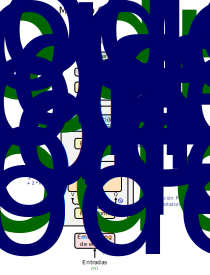
\includegraphics[width = 0.55\textwidth]{\DirFigCdos/Qwen3}
    \caption{Arquitectura \textit{Qwen3}.}
    \label{fig:qwen3}
\end{figure}

La arquitectura MoE fue inicialmente propuesta por Shazeer et al.
\cite{shazeer_outrageously_2017} y empleada con \textit{transformers} por Du et al. \cite{du_glam_2022}. Esta arquitectura
consiste en reemplazar las capas de alimentación directa (\textit{feedforward}) del
transformer por un bloque MoE. Este bloque se compone de múltipes capas de alimentación directa
en paralelo, llamadas expertos, conectadas a un enrutador o compuerta que ``escoge'' los expertos más
aptos para procesar el token de entrada, como se muestra en la figura \ref{fig:moe}. Esta
arquitectura permite entrenar modelos con más parámetros pero a un menor costo computacional
pues solo una parte de los parámetros se activa en cada paso.

\begin{figure}
    \centering
    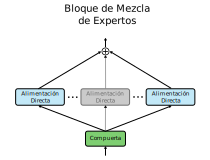
\includegraphics[width = 0.55\textwidth]{\DirFigCdos/MoE}
    \caption{Arquitectura \textit{Mezcla de Expertos}.}
    \label{fig:moe}
\end{figure}

Además del modelo Qwen3 en su versión MoE, otro modelo que se beneficia de
esta arquitectura es el modelo GPT-OSS. Este modelo es un modelo de licencia
abierta, basado en GPT-2 y GPT-3, liberado por OpenAI en dos versiones: 20B y 120B.
Cuenta con bloques MoE de 32 y 128 expertos para cada versión, escogiendo los
top-4 expertos para procesar cada token y emplea SwiGLU en las capas de alimentación directa.
La arquitectura se presenta en la figura \ref{fig:gpt_oss}.

\begin{figure}
    \centering
    \includegraphics[width = 0.55\textwidth]{\DirFigCdos/GPT-OSS}
    \caption{Arquitectura \textit{GPT-OSS}.}
    \label{fig:gpt_oss}
\end{figure}

\subsection{Modelos de representaciones vectoriales \textit{embeddings}}

Se llama \textit{embedding} a una representación numérica de una secuencia de
caracteres, que puede ser una palabra o una oración completa. La característica
principal de un \textit{embedding} es que las palabras similares tienen
representaciones similares, mientras que palabras u oraciones diferentes u
opuestas tienen \textit{embeddings} muy distintos. A los modelos con la capacidad
de generar representaciones con estas características se les conocen como modelos
de \textit{embeddings}.

Existe una gran variedad de modelos para generación de \textit{embeddings}, por ejemplo,
el modelo SBERT tiene la capacidad de extraer \textit{embeddings} de oraciones
completas, considerando la posición y contexto de las palabras, permitiendo
generar representaciones más significativas \cite{reimers_sentence-bert_2019}.
Otro modelo relevante es el modelo \textit{Qwen3-Embedding} \cite{zhang_qwen3_2025},
el cual es una versión de Qwen3 que fue sometida a un proceso de ajuste fino
en tareas como la similitud semántica o la respuesta a preguntas con
conjuntos de datos generados sintéticamente y obtiene representaciones
orientadas a la tarea que se desea realizar.

\subsection{Cuantización de modelos}

La cuantización consiste en reducir el uso de memoria de un LLM mediante el uso
de pesos que utilicen representaciones de menor precisión, esto permite el
despliegue de modelos grandes en hardware de menor tamaño \cite{egashira_exploiting_2024}.
Algunos de los métodos de cuantización relevantes para este proyecto son la
cuantización a formato MPFX4 \cite{rouhani_ocp_nodate} que reduce el tamaño de los
parámetros a 4.25 bits por parámetro, y las cuantizaciones Q4\_K\_M y Q8\_0
que reducen el tamaño a 4 bits y 8 bits por parámetro respectivamente.

\subsection{Modelos comerciales}

Se entiende por modelos comerciales a aquellos que pertenecen a una entidad
privada y su uso está restringido por el pago de una subscripción.
Además, la arquitectura del modelo, métodos de entrenamiento, así como sus
parámetros de funcionamiento no son públicos. Algunos ejemplos son ChatGPT
(OpenAI), Gemini (Google), Claude (Anthropic), entre otros. Usualmente los
proveedores de estos modelos lo hacen a través de aplicaciones web o APIs,
y en ocasiones, cuentan con versiones gratuitas con capacidades limitadas.

\subsection{Modelos de código abierto}

Los modelos de código abierto son aquellos que se encuentran disponibles
en sitios especializados, tanto su arquitectura como parámetros de
funcionamiento son accesibles, usualmente a través de una licencia de uso
que no es restrictiva. Algunos ejemplos son DeepSeek (DeepSeek),
Llama (Meta), Qwen (Qwen), entre otros. Los creadores de estos modelos
generalmente no proveen aplicaciones web o APIs, sino que permiten que los
usuarios o desarrolladores los utilicen en sus propias infraestructuras,
sin depender del creador.

\section{QA con modelos multidominio}

Un modelo multidominio tiene la capacidad de responder preguntas que se
le hagan en lenguaje natural y emitir respuestas que usualmente son también
en lenguaje natural, pero pueden ser de otra naturaleza.

\subsection{Respuestas desde conocimiento previo}

Durante el entrenamiento del modelo, éste se entrena con corpus de información
muy grande y de diversas fuentes, además de que se le hace un ajuste fino
para esta tarea, de tal forma que el modelo es capaz de responder una pregunta
utilizando la información que se le proporcionó durante su entrenamiento.

Este tipo de respuestas es buena cuando se trata de preguntas de dominio abierto
donde la información es pública y no cambia con el tiempo, como es el caso
de conocimientos generales o eventos históricos. Sin embargo, las respuestas suelen ser deficientes
cuando se trata de eventos recientes, situaciones personales o conocimiento
restringido, en estos casos se pueden presentar alucinaciones, que son
respuestas cuya estructura es correcta, pero su información es errónea. Además,
los modelos no cuentan con la capacidad de indicar la fuente de la información.

\subsection{Respuestas desde un contexto}

Es posible alimentar un modelo con información desde la cual pueda buscar o
inferir la respuesta, a esta información se le denomina contexto y usualmente
se trata de un texto del cual se puede extraer la respuesta. Un ejemplo es
proporcionar la información biográfica de una
persona como contexto y hacer preguntas sobre la persona. Generalmente,
estas respuestas son más acertadas, pues los modelos son entrenados
para responder preguntas de esta forma, siempre y cuando el contexto sea adecuado. Una
desventaja de este método es que los modelos operan con ventanas de contexto
limitadas, las cuales pueden ser de algunos miles de tokens hasta unos pocos
millones y es posible que el contexto que se deba proporcionar sea mayor.

\section{Recuperación-Generación Aumentada (RAG)}

Para superar las limitantes que presentan los LLMs, el uso de técnias de
de Recuperación-Generación Aumentada (RAG, Retrieval-Augmented Generation) ha
sido incorporado con frecuencia. Estas técnicas consisten en incorporar
información o conocimiento desde fuentes de datos externas, que sirven como
complemento a las preguntas \cite{fan_survey_2024}. Un esquema de RAG simple,
como el que se presenta en la figura \ref{fig:rag},
contempla tres etapas principales: indexado, recuperación y generación

\begin{figure}
    \centering
    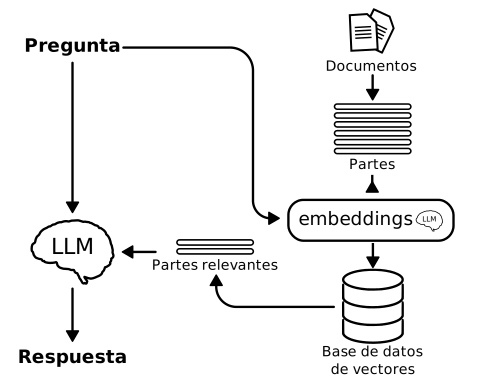
\includegraphics[width = 0.5\textwidth]{\DirFigCdos/simple_rag}
    \caption{Diagrama de funcionamiento de un esquema de RAG simple.}
    \label{fig:rag}
\end{figure}

\subsection{Indexado}

En su forma más simple, una base de conocimiento para RAG parte de la recolección
de documentos relacionados con las preguntas que se harán a continuación.
Una de las ventajas es que no hay limitante en la cantidad o tamaño de
los documentos, aunque si deben estar en formato de texto.
Estos documentos se separan en framentos, comúnmente
llamados \textit{chunks}, el objetivo es obtener fragmentos pequeños pero
que contengan suficiente información. Posteriormente se calcula la
representación vectorial (\textit{embedding}) de cada framento, para finalmente
almacenar cada fragmento con su respectivo \textit{embedding} en una base
de datos.

\subsection{Recuperación}

Cuando se le hace una solicitud al LLM, la recuperación consiste
en buscar información relevante, en forma de fragmentos de
documentos, en la base de datos previamente construida. La forma de
determinar si un fragmento es relevante o no para la pregunta es calculando la
similitud entre la solicitud y el fragmento. Una vez calculada la
similitud con todos los fragmentos disponibles, se seleccionan los \textit{k}
fragmentos más similares o se establece un valor umbral y se consideran
como relevantes aquellos que estén por encima del umbral. Uno de los cálculos de distancia
más comunes es la distancia coseno, en su forma de similitud coseno, como se muestra en la
ecuación \ref{eq:cos_similarity}

\begin{equation}\label{eq:cos_similarity}
    d = 1.0 - \frac{\sum{(A_i \times B_i)}}{\sqrt{\sum{(A_i^2)}}\sqrt{\sum{(B_i^2)}}}
\end{equation}

Otra métrica común es el cálculo de similitud empleando el producto interno,
como se muestra en la ecuación \ref{eq:inner_product}.

\begin{equation}\label{eq:inner_product}
    d = 1.0 - \sum{(A_i \times B_i)}
\end{equation}

\subsection{Generación}

En esta etapa, tanto la solicitud como los documentos seleccionados son
sintetizados en una instrucción coherente que se le proporciona al modelo.
Usualmente esta instrucción incluye: indicación de responder la pregunta
solamente con los fragmentos proporcionados, los fragmentos de texto y la
pregunta.

\section{Reentrenamiento de los modelos}

Tanto los LLMs comerciales como los de código abierto pasan por una serie de
pasos de entrenamiento y ajuste para funcionar adecuadamente en los
diferentes dominios para los que son preparados, sin embargo, es
posible mejorar su rendimiento en tareas más específicas aplicando diferentes
técnicas de ajuste.

\subsection{Ingeniería de instrucciones (\textit{prompts})}

Cuando un modelo está entrenado para seguir instrucciones, es posible modificar
su comportamiento dando instrucciones adicionales que le sirvan como guía
al momento de dar la respuesta, a esto se le conoce como ingeniería de \textit{prompts}.
Con esta técnica se puede instruir al modelo a realizar una serie de pasos
antes de emitir la respuesta, modificar el tono, longitud o intención de la
respuesta, además de proporcionar información sobre la situación en que
se debe desempeñar.

\subsection{Ajuste fino supervisado}

Consiste en tomar un conjunto de datos que contenga ejemplos del comportamiento que
se desea que aprenda el modelo. En este proceso suelen usarse
ejemplos con pares instrucción-respuesta, donde la respuesta tiene
las características que se desea que el modelo aprenda. Existen diferentes
ténicas para llevar a cabo este proceso, que van desde reajustar todos los pesos
del modelo, hasta emplear técnicas como LoRA (Low-Rank Adaptation) que congela
el modelo preentrenado y solo entrena un pequeño número de parámetros adicionales.

\subsection{Aprendizaje por refuerzo}

El aprendizaje por refuerzo consiste en entrenar al modelo para tomar decisiones
que maximicen una recompenza. En el caso de los modelos de lenguaje, uno
de los enfoques más utilizados es el aprendizaje por refuerzo con
retroalimentación humana (RLHF, Reinforcement Learning from Human Feedback),
el cual utiliza retroalimentación humana para optimizar modelos. Esta
técnica de ajuste es particularmente útil porque es posible hacer que
el modelo adquiera comportamientos que no son fáciles de modelar matemáticamente,
sin embargo, tiene la desventaja de que requiere intervención humana y es por
ello más lento.

\section{Documentos normativos}

Se entiende como documentos normativos a aquellos que contienen reglas o
normas que rigen la operación de una organización o un organismo dentro de la
misma, también pueden ser reglamentos de eventos o actividades específicas.
En la actualidad, la mayoría de los documentos normativos se encuentran
digitalizados en formato PDF y, en ocasiones, disponibles
en servidores web para que los miembros de las organizaciones puedan consultarlos
en cualquier momento.

En el caso de la normativa de la Universidad de Guanajuato, y de muchas otras
normativas, la estructura de los documentos se divide principalmente en:
Título, Sección, Capítulo y Artículos. Este trabajo pretende aprovechar esta
estructura predefinida para obtener mejores fragmentos de documentos para la
metodología RAG y para referenciar las repuestas del sistema.

\subsection{Formato PDF}

El formato PDF (Portable Document Format) es un formato creado con el objetivo de
ofrecer una forma sencilla y segura de presentar e intercambiar documentos con
independencia del software, hardware o sistema operativo que utilice quien
los consulte. Con este fin, el formato PDF se encuentra estandarizado por la
ISO (Organización Internacional de Normalización) bajo la ISO 32000-1:2008
(PDF 1.7) y más recientemente la ISO 32000-2:2020 (PDF 2.0). Sin embargo,
este formato fue pensado como una herramienta para presentar
documentos en una forma entendible por humanos, es decir, no está
diseñado para que una máquina interprete su contenido de forma sencilla, lo
cual dificulta el procesamiento automático del mismo.

\subsection{Herramientas de extracción de texto}

Los LLMs operan con entradas de texto, si los documentos a ser empleados
se encuentran en formato PDF es necesario extraer la información textual que
contienen. Existen diferentes herramientas para extraer el texto de documentos PDF,
sin embargo, el resultado suele presentar errores o limitaciones propias del formato,
como son la presencia de encabezados y pies de página entre el contenido
del documento, la falta de distinción entre títulos, subtítulos o divisiones
de secciones y la dificultad para leer tablas.

En el Apéndice A se encuentra una lista de las herramientas más comunes y
sus limitantes, la cual se emplea para seleccionar la herramienta más apta.
Dependiendo de la herramienta a emplear se debe hacer un procesamiento del
archivo PDF para eliminar los defectos e información que no sea relevante,
este proceso se presenta como parte de la metodología del proyecto.

\section{Trabajos relacionados}

En un esfuerzo por implementar una arquitectura robusta de QA
desde diferentes fuentes de información, Christmann \& Weikum
\cite{christmann_rag-based_2024} presentaron el sistema QUASAR, el cual emplea una
arquitectura basada en RAG para responder preguntas desde texto sin estructura,
tablas y grafos de conocimiento. Este sistema procesa las preguntas en
diferentes etapas, que denomina: entendimiento de la pregunta, recuperación
de evidencia y reclasificación y filtrado. Con esta metología alcanzó
resultados superiores a modelos grandes como GPT-4 y Llama 3 en los benchmarks
CompMix \cite{christmann_compmix_2024} y TimeQuestions \cite{jia_complex_2021}
con un modelo Llama 3.1-8B-instruct\footnote{https://huggingface.co/meta-llama/Llama-3.1-8B-Instruct}.

Al ser sistemas basados en RAG, este proyecto comparte elementos comunes
con el sistema QUASAR, sin embargo, se diferencía en que pretende aprovechar
la estructura semi-estandarizada de los documentos normativos para realizar
una fragmentación más eficiente de los documentos. Además, la restricción
del dominio de las preguntas a documentos específicos, permite construir
una base de datos de conocimiento más simple, tanto en tamaño como en
pasos de procesamiento, lo que da como resultado un sistema más rápido y compacto.

Uno de los problemas principales del RAG es la recuperación de fragmentos
relevantes de los documentos. Trabajos como el de Shao et al. \cite{shao_enhancing_2023}
se centran en proponer mejores técnicas en la identificación de
documentos relevantes en grandes volúmenes de datos, aplicando una
sinergia entre el recuperador y el generador con el fin de mejorar las respuestas
de manera iterativa. Por su parte, Shi et al. \cite{shi_replug_2024} proponen el
\textit{framework RePlug}, que consiste en tratar al modelo de lenguaje
que responde la pregunta como una caja negra y reentrenar el modelo
responsable de la recuperación de información para optimizar su desempeño.
Dadas estas consideraciones, el sistema propuesto en este proyecto incluye una etapa de ajuste
fino para el modelo que obtiene los \textit{embeddings} de los documentos.

Por último, existen herramientas comerciales y de código abierto con la
capacidad de ejecutar metodologías RAG para responder a preguntas de documentos,
siendo el más usado ChatGPT\footnote{https://help.openai.com/en/articles/8868588-retrieval-augmented-generation-rag-and-semantic-search-for-gpts},
el cual permite generar chats personalizados
y proporcionar una serie de documentos como contexto. Al habilitar la opción
de ``Recuperación de conocimiento'' la herramienta aplica RAG y responde
las preguntas correspondientes. Otra heramienta con características
similares es LMStudio\footnote{https://lmstudio.ai/docs/app/basics/rag},
la cual es de código abierto y permite el uso de
diferentes modelos, así como su ejecución en entornos locales.

A pesar de las bondades de las herramientas existentes, éstas
ponen sobre el usuario la responsabilidad de encontrar los documentos
requeridos y proporcionarlos al sistema. Además, tienen un límite a la cantidad de
documentos de consulta y, cuando el historial de conversación crece demasiado,
se debe reiniciar el chat y repetir el proceso. Otras desventajas incluyen la
imposibilidad de referenciar sus respuestas a los artículos específicos, así
como la presencia de texto no deseado, como encabezados, pies de página o
malas interpretaciones de la secuencia del texto. Son estos problemas los
que se busca resolver en este proyecto, al proporcionar
una herramienta que esté lista para usarse, sea de código abierto, proporcione
respuestas referenciadas correctamente y permita un nivel de personalización
completo para la institución.
